\documentclass[12pt,a4paper]{article}
\usepackage[a4paper,textwidth=170mm,textheight=245mm]{geometry}
\usepackage[utf8]{inputenc}
\usepackage{fancyhdr}
\usepackage{datetime2}
\usepackage{parskip}
\usepackage{amsmath}
\usepackage{float}
\usepackage{graphicx}
\usepackage{wrapfig}

% For the wrapfigure
\usepackage{caption}
\usepackage{subcaption}

\graphicspath{{plots/}}

\renewcommand{\figurename}{Figur}

\pagestyle{fancy}
\fancyhf{}

\lhead{TANA09 - Datatekniska beräkningar}
\rhead{\today}
\setlength{\headheight}{15pt}

\cfoot{\thepage}

\begin{document}

\begin{center}
	\Huge
	\textbf{Sammanfattning}
	\\
	\large
	Michael Sörsäter
\end{center}

\large
\section{Fel}
Typer av fel:
\begin{itemize}
\item{$R_X$ fel i resultatet, som härrör från fel i indata}
\item{$R_{XF}$ fel i resultatet, som härrör från fel i de använda funktionsvärdena}
\item{$R_B$ avrundningsfel}
\item{$R_T$ trunkeringsfel}
\end{itemize}

Närmevärde till x: $\bar{x}$

Absolut fel: $\Delta x = \bar{x}-x$

Relativt fel: $ \frac{\Delta x}{x}$

\subsection{Korrekta decimaler} \label{korrekta}
Om $|\Delta a| \leq 0.5*10^{-t}$ sägs $\bar{a}$ ha t korrekta decimaler

\subsection{Fortplantning av fel}
\begin{table}[H]
	\Large
  \centering
  \begin{tabular}{| l | l | l | l |}
  	\hline
  	Beräkning & Absolut Fel & Relativt fel & Felgräns \\ \hline
  	$ y = x_1 + x_2 $ &
  	$\Delta y = \Delta x_1 + \Delta x_2 $ &
  	&
  	$| \Delta y| \leq |\Delta x_1| + |\Delta x_2|$ \\ \hline

	$ y = x_1 - x_2 $ &
	$ \Delta y = \Delta x_1 - \Delta x_2 $ &
	&
	$| \Delta y| \leq |\Delta x_1| + |\Delta x_2|$\\ \hline

  	$ y = x_1 * x_2 $ &
  	&
  	$ \frac{\Delta y}{y} \approx \frac{\Delta x_1}{x_1} + \frac{\Delta x_2}{x_2} $ &
  	$| \frac{\Delta y}{y} | \leq \approx | \frac{\Delta x_1}{x_1} | + | \frac{\Delta x_2}{x_2} |$ \\ [10pt]\hline

	$ y = x_1 / x_2 $ &
	&
	$ \frac{\Delta y}{y} \approx \frac{\Delta x_1}{x_1} - \frac{\Delta x_2}{x_2} $ &
	$| \frac{\Delta y}{y} | \leq \approx | \frac{\Delta x_1}{x_1} | + | \frac{\Delta x_2}{x_2} |$ \\ [10pt]\hline

  \end{tabular}
  \caption{Fortplantning av fel}
\end{table}

\newpage
\subsection{Maximalfelsuppskattning}
För att uppskatta felet när en dator räknar utförs beräkningsanalys på varje del.
Följande summa skrivs upp:

$$ | \Delta f| \leq \approx \sum_{k=1}^{n} | \frac{\delta f}{\delta x_k} \Delta x_k| $$

Varje beräkning (+,-,*,/\ldots) ersätts av en bokstav.
Derivatan beräknas med avseende på sin bokstav:

$|\Delta f| \leq |\frac{\delta f}{\delta a}| |\Delta a|
|\frac{\delta f}{\delta b}| |\Delta b| \ldots$

För att uppskatta absoluta felet utnyttjas ($\mu =$ maskinkonstant):

$ \frac{\Delta a}{a} \approx \mu \Leftrightarrow \Delta a \approx a\mu$



\section{Talsystem och flyttalsrepresentation}
Talsystem beskrivs på formen $(\beta, t, L, U)$
\begin{itemize}
	\item{$\beta$ är basen}
	\item{t är precisionen (antalet decimaler)}
	\item{L är undre gränsen på exponenten}
	\item{U är övre gränsen på exponenten}
\end{itemize}

Med 32 bitar representeras ett flyttal som:
(2, 23, -126, 127)

s (1 bit) positivt/negativt \\
e (8 bitar) exponenten för talet \\
f (23 bitar) decimaldelen för talet \\
\Large
$$ x = (-1)^s(1.f)_2*2^{e-127} $$
\large

Felet från det talet man lagrar till det riktiga talet:

\Large
$$ \frac{|x-x_r|}{|x|} \leq \frac{1}{2}\beta^{-t}$$
\large
där $x_r$ är det talet som ligger närmast x.

Jämför med formeln i \ref{korrekta}.

\subsection{Roten ur}
För att beräkna roten ur av ett tal. $ x = \sqrt{a}$ används funktionen $ f(x) = x^2 - a$.

Med Newton-Raphsons fås:
$ x_{n+1} = \frac{1}{2}(x_n-\frac{a}{x_n})$

I flyttalssystemet skrivs tal som:

$$ x = (1.f)_2 2^e \Rightarrow \sqrt{x} = \sqrt{(1.f)_2} \sqrt{2^e} $$

Resulterar i två fall:

\Large
$$
\sqrt{2^e} = \begin{cases}
               e\, \text{jämn}, 2^{\frac{e}{2}}\\
               e\, \text{udda}, \sqrt{2}\;2^{\frac{e-1}{2}}
            \end{cases}
$$

\large
Termen $(1.f)_2$ ligger alltid i intervallet $[1,2]$. Då e är udda, multipliceras tvåan in i den roten och uttrycket blir:

$$ \sqrt{x} = \sqrt{(1.f)_2 2}\;2^{\frac{e-1}{2}} $$

Vilket göra att samma term ligger i intervallet $[1,4]$ och det blir då det enda intervallet som måste beräknas.




\section{Summa - restterm}
Summa som är konvergent

$$ S = \sum_{n=1}^{\infty} a_n, \;
 S_N = \sum_{n=1}^{N} a_n$$
$$ R_N = S - S_N = \sum_{n=N+1}^{\infty} a_n $$

Hur uppskattas $R_N$ utan att räkna ut den?

\subsection{Alternerande}
Är serien konvergent och alternerande:

$$ |R_N| \leq |a_{N+1}|$$
Alltså, felet är mindre än nästa term.

\subsection{Postiv monotont avtagande}
Om funktionen avtar, går mot 0.
$$ R_N = \sum_{N+1}^{\infty} f(n) \leq \int_{N}^{\infty} f(x) dx $$
Alltså, integrera funktionen och beräkna integralen.
Lägg märke till att man beräknar en extra term då man i integralen börjar på N istället för N+1.

\section{Iterationsmetoder}
\subsection{Konvergerar}
För att undersöka om en iterationsmetod konvergerar mot en lösning med ett givet startvärde $x_0$ måste den uppfylla två krav:
\begin{enumerate}
	\item{Måste kunna skrivas om på originalform}
	\item{$ |\varphi' (x_0) | < 1 $ för att den ska konvergera}
\end{enumerate}
Exempel:

$ f(x) = xe^x-1 = 0 $

$ x_{n+1} = \underbrace{\frac{1 + x_n}{1 + e{x_n}}}_\text{$\varphi(x)$}$

Genom att multiplicera upp nämnaren och flytta runt fås samma orginalfunktion (krav 1). Genom att derivera och sätta in $x_0$ fås ett värde som är $< 1$ (krav 2).

\subsection{Newton-Raphsons metod}
$$ x_{n+1} = x_n - \frac{f(x_n)}{f'(x_n)}, \: n = 0,1,2,\ldots $$

\subsection{Metodoberoende feluppskattning}
Används för att uppskatta hur nära x är $x^*$.

$$ |x^{*}-\bar{x}| \leq \frac{f(\bar{x})}{f'(\bar{x})} $$

\newpage
\section{Interpolation och splines}
\subsection{Interpolation}

Beräkna polynomet:

$$ p_n(x) = c_0 + c_1(x-x_1) + c_2 (x-x_1)(x-x_2) + \ldots $$

Beräkna konstanterna C genom att först sätta in $x_1$ (gör alla delar till 0 förutom $c_0$) och sedan vidare likadant.

Felet är den ``Extra term'' som inte ingår i interpolationen, $R_T$.
För en linjär interpolation är det termen vid $c_2$.

Vid en fullständig feluppskattning ska tre delar tas med.
Alla delar är absolutbelopp.

\begin{itemize}
\item{$R_B$ Avrundningsfel.
Efter beräkningen P(a), har svaret t korrekta decimaler. \\Ger felet: $ R_B = 0.5 * 10^{-t}$}
\item{$R_T$ Trunkeringsfel.
(är ofta den dominerande delen)
Använd termen $c_n$ för att beräkna felet.
Ex: $ R_T \leq |c_2 (x-x_1)(x-x_2)|$
}
\item{$R_{XF}$ Fel i indatan.
Likadant som för $R_B$ antalet t decimaler som lägst givna i indatan.
$R_{XF} = 0.5 * 10^{-t}$}
\end{itemize}

Svaret blir sedan $R_{TOT} = | R_B | + | R_T | + |R_{XF}| $

\subsubsection{Fel indata}
Ibland har även den punkt som uppskattas en felmarginal:

$A = \bar{A} \pm \Delta A $

Vad blir felet i $f(A)$?

Använd maximalsfelsuppskattning.

$|\Delta f| \leq |\frac{\delta f}{\delta A}| |\Delta A| \approx |\frac{\delta P_n}{\delta x}| |\Delta A| \approx \left. \middle/ \text{om linjär} \middle/ \approx \right. |c_1||\Delta A|$


\subsection{Spline}
Låt
$$ a = x_1 < x_2 < \ldots < x_n < b $$

\subsection{Lineär spline}
En funktion s sägs vara en lineär splinefunktion på intervallet [a,b] om:
\begin{itemize}
\item{s är kontinuerlig på [a,b]}
\item{s är en rät linje på varje delintervall $[x_i,x_{i+1}], i = 1,\ldots,n-1 $}
\end{itemize}

\subsection{Kubisk spline}
En funktion s sägs vara en kubisk splinefunktion på intervallet [a,b] om:
\begin{itemize}
\item{s, s', s'' är kontinuerlig på [a,b]}
\item{s är ett polynom av grad $\leq 3$ på varje delintervall $[x_i,x_{i+1}], i = 1,\ldots,n-1 $}
\end{itemize}

Finns två typer av kubiska splines.
Antingen är derivatan i ändpunkterna 0 (rak linje), eller så knyter den ihop med nästa spline.
För formler om hur man formeln är, se sida 130 i kursboken.

\begin{figure}[H]
    \centering
    \begin{subfigure}[b]{0.45\textwidth}
        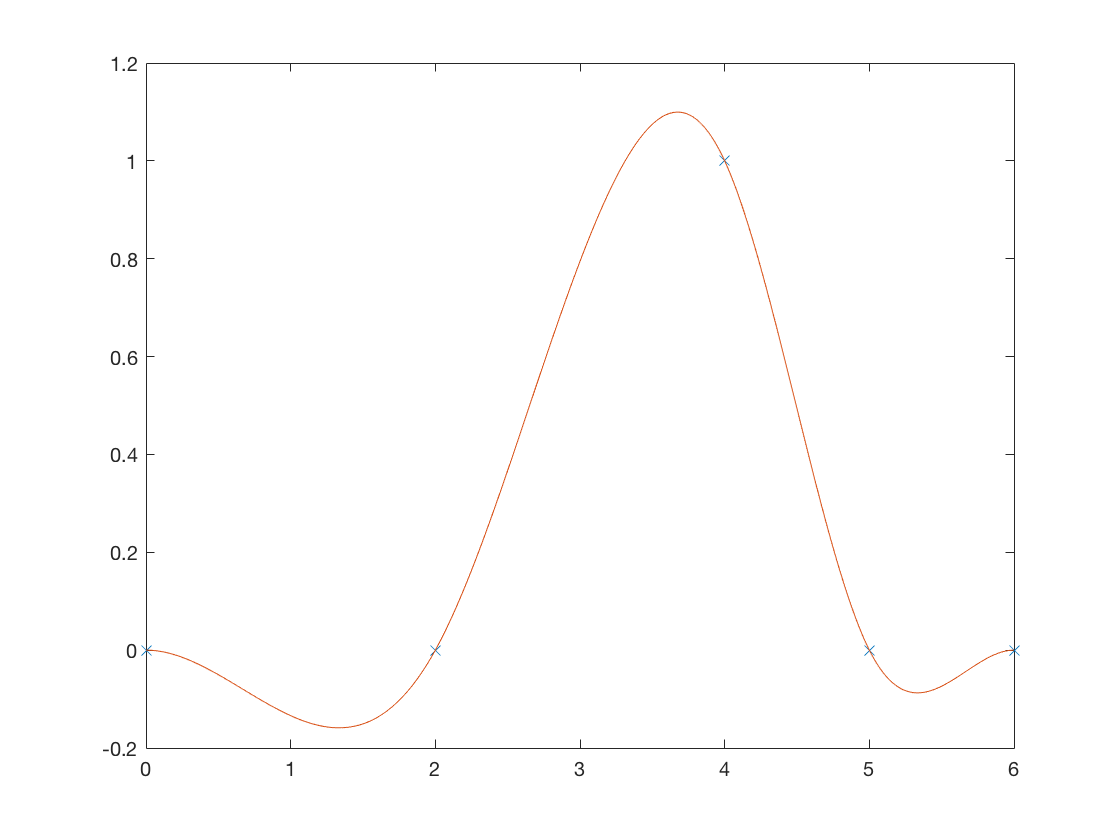
\includegraphics[width=\textwidth]{3-2}
        \caption{Derivatan 0}
    \end{subfigure}
    ~ % spacing
    \begin{subfigure}[b]{0.45\textwidth}
        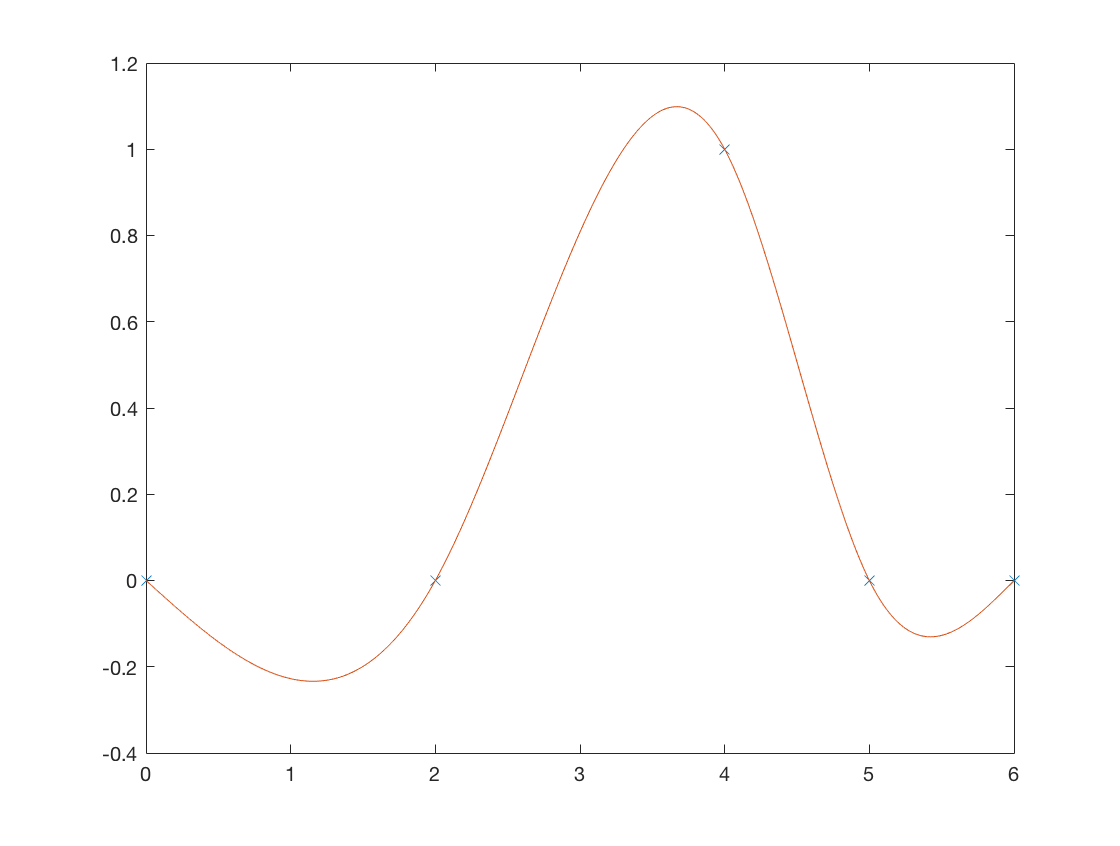
\includegraphics[width=\textwidth]{3-1}
        \caption{Mjuk övergång till nästa spline}
    \end{subfigure}
    \caption{Kubiska Splines}
\end{figure}

\newpage
\section{LU-faktorisering}
Från matrisen A, beräkna $PA=LU$ där P är en permutationsmatris (ändrar om raderna).

$P_{12} =
\begin{pmatrix}
0 & 1 & 0 \\
1 & 0 & 0 \\
0 & 0 & 1
\end{pmatrix}
,
L =
\begin{pmatrix}
1 & 0 & 0 \\
a & 1 & 0 \\
b & c & 1
\end{pmatrix}
,
U =
\begin{pmatrix}
a & b & c \\
0 & d & e \\
0 & 0 & f
\end{pmatrix}
$

Används för att kunna lösa Ax=b.

$Ax = b \Leftrightarrow PAx = Pb \Leftrightarrow LUx = Pb$

Sätt $Ux = y$, lös $Ly = Pb$ och sedan $Ux = y$

\section{Feluppskattning Ax = b}
$\frac{||\Delta x||_\infty}{||x||_\infty} \leq ||A||_\infty ||A^{-1}||_\infty \frac{||\Delta b||_\infty}{||b||_\infty}$

Matrisnormen defineras som:

$ ||A||_\infty = \underset{1 \leq i \leq n}{\max} ( \sum_{j=1}^n |a_{ij}|)$

Alltså, för varje rad, ta absolutvärdet av varje element och addera dem. Maximala värdet för alla rader är matrisnormen.

Matrisnormen är ett mått på hur störningar i högerledet (b) förstoras och påverkar x.

\section{Minsta kvadratmetoden}
Minsta kvadratmetoden används för att hitta en modell för data som inte har exakta lösningar.

För att lösa ekvationen $ Ax = b$ används $A^T$ för att skapa normalekvationen:

$$ A^TAx = A^Tb $$

Det går att visualisera det som att det finns ett plan som spänns upp av kolonnerna i A och en vektor b, som ej ligger i planet. Vi vill då hitta en vektor, x, som placeras ortogonalt mot b (vilket då är närmast). För att ``få ner'' b i planet multipliceras b med matrisen $A^T$ och då även vänsterledet. Detta resulterar i normalekvationen, som alltid har en lösning.

\section{Deriveringsregler}
$\frac{d}{dx}\frac{u}{v} = \frac{vu'-uv'}{v^2}$

\section{Taylor \& Maclaurin}

\LARGE
$ e^x = \sum_{n=0}^{\infty} \frac{x^n}{n!} = 1 + x + \frac{x^2}{2!} + \frac{x^3}{3!} + \ldots $

$ sin(x) = \sum_{n=0}^{\infty} \frac{(-1)^n}{(2n+1)!} x^{2n+1} = x - \frac{x^3}{3!} + \frac{x^5}{5!} - \frac{x^7}{7!} + \ldots$

$ cos(x) = \sum_{n=0}^{\infty} \frac{(-1)^n}{(2n)!} x^{2n} = 1 - \frac{x^2}{2!} + \frac{x^4}{4!} - \frac{x^6}{6!} + \ldots$

$ f(x+h) = \sum_{n=0}^{\infty} \frac{f^n(x)}{n!}h^n = f(x) + f(x)h + \frac{f^{(2)}(x)}{2!}h^3 + \ldots $

\end{document}
